\subsubsection{RANSAC-Based Motion Filtering}
A key stage in the pipeline is filtering static landmarks from dynamic objects to ensure ego-motion estimation is based only on stable references.  
To achieve this, a RANSAC-based model is fitted to the relationship between azimuth angle $\theta$ and Doppler velocity $v_d$.

\paragraph{Principle and Theory}
Static reflections observed by a moving radar follow a predictable Doppler pattern:
\[
v_d = v_e \cos(\theta),
\]
where $v_e$ is the vehicle’s forward velocity.  
Objects directly in front exhibit $v_d \approx v_e$, while those at $90^\circ$ azimuth have $v_d \approx 0$, and intermediate azimuths form a smooth curve.  
Dynamic targets deviate from this distribution, appearing as outliers.  

Figure~\ref{fig:ransac_simulated_static_dynamic} illustrates this concept using simulated data.

\begin{figure}[!htbp]
    \centering
    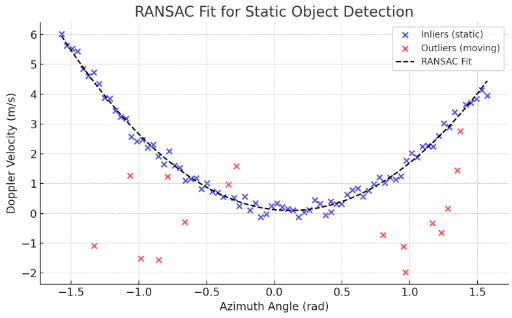
\includegraphics[width=0.9\linewidth]{images/RANSAC.png}
    \caption{Simulated data: RANSAC fit of Doppler vs.\ azimuth. Inliers = static (blue), Outliers = moving (red).}
    \label{fig:ransac_simulated_static_dynamic}
\end{figure}

\paragraph{Implementation}
In practice, directly fitting the cosine model requires prior knowledge of $v_e$, which is not yet available at this stage of the pipeline.  
Instead, a polynomial approximation is used:
\[
v_d = a\theta^2 + b\theta + c,
\]
fitted with \textbf{RANSACRegressor}.  

The algorithm iteratively:
\begin{enumerate}
    \item Samples small subsets of $(\theta, v_d)$ pairs.
    \item Fits a quadratic model.
    \item Evaluates inliers based on residual error.
    \item Selects the model with maximum consensus.
\end{enumerate}

This approach bends the quadratic to approximate the Doppler distribution of static objects, which in the radar's limited FOV resembles half of a cosine curve.  
Inliers are classified as static reflections, while outliers correspond to dynamic objects that must be excluded from ego-motion estimation.

\begin{figure}[!htbp]
    \centering
    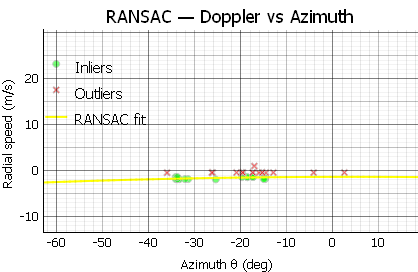
\includegraphics[width=0.9\linewidth]{images/RANSAC_movingTarget_wPtCloud.png}
    \caption{Real implementation of RANSAC filtering: green = static inliers, red = dynamic outliers.}
    \label{fig:ransac_real_static_dynamic}
\end{figure}

\paragraph{Pipeline Role}
As illustrated in the system pipeline (Fig.~\ref{fig:dual_radar_pipeline}), the RANSAC filter is positioned after static thresholding and before ego-velocity estimation.  
Its primary purpose at this stage is to separate dynamic objects from static landmarks, ensuring that subsequent modules operate only on consistent and reliable data.  

Without this step, moving objects would propagate through clustering and ICP, corrupting the estimation of ego-motion.  
By filtering out dynamic outliers, RANSAC guarantees that only stable reflections are retained for trajectory alignment and speed estimation.  
\vspace{2.0em}
\\
The output of this stage is therefore two-fold:
\begin{itemize}
    \item A refined set of static landmarks, which serve as input for clustering and ICP-based odometry,
    \item A clean separation of dynamic actors, preventing them from biasing ego-motion estimation.
\end{itemize}
